\section{Proposed Method}

In this method, we propose to enhance the bag-of-words model for text classification by presenting a novel regularizer which would assign similar coefficients to words used in similar context.

\begin{figure}
\centering
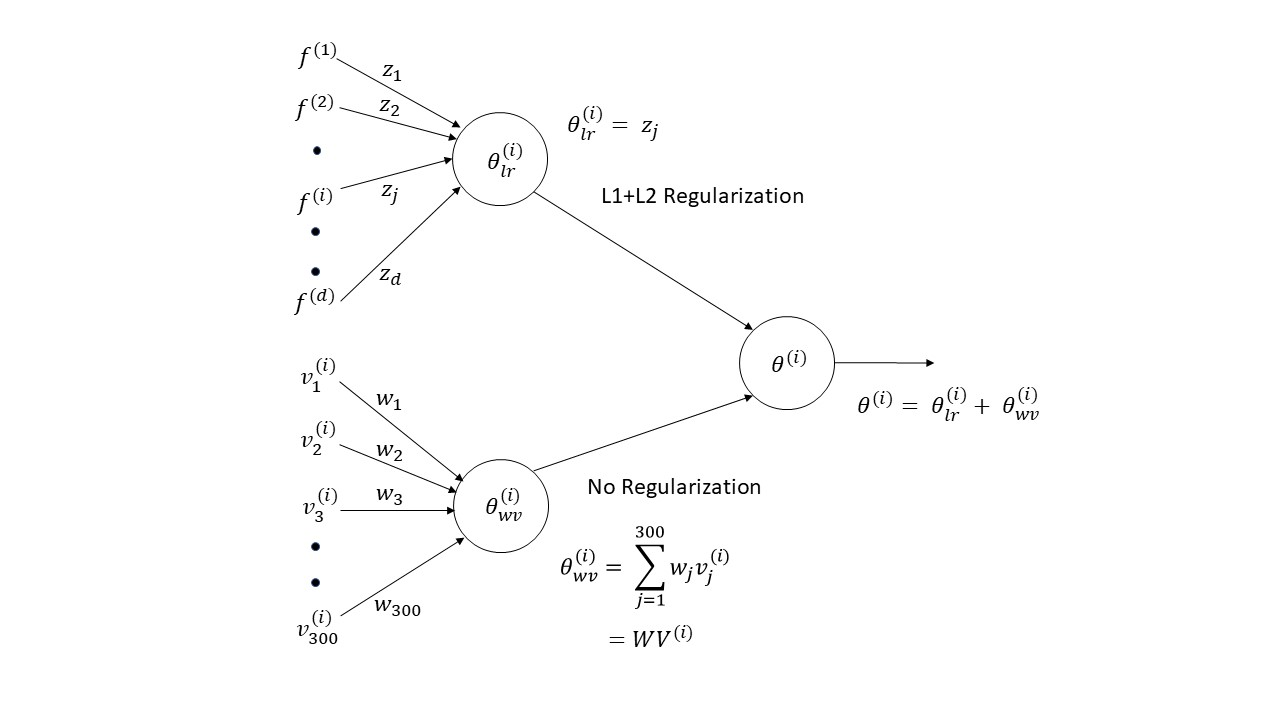
\includegraphics[width=18cm, height=10cm]{images/Fig3.jpg}\\
\centering
\caption{Network diagram to learn $\theta^{(i)}$ from word$_{i}$ representation f(v$^{(i)}$)}
\label{fig:foo}
\end{figure}

Formally, the problem we are trying to solve can be formulated as follows: Given a set of m documents with n features, the documents would be represented by matrix X $\in$ R$^{m x n}$. We want to find the coefficients that predict the output Y from the documents X and we want to build a model where the coefficients ($\theta^{(i)}$) are a function of its word$_{i}$ representation ($v^{(i)}$), i.e.,

\begin{equation}\label{lb1}
\theta^{(i)} = f(v^{(i)})
\end{equation}

This would act as a regularization constraint so that similar word representations would have similar coefficients, which satisfies a continuity condition

\begin{equation}
|f(v^{(1)}) - f(v^{(2)}))|\ \leq\ sim(v^{(1)}, v^{(2)})
\end{equation}

where, $sim$ dictates the similarity between words $v^{(1)}$ and $v^{(2)}$ and $ f(v^{(1)}), f(v^{(2)})$ are coefficients of their respective words as per (\ref{lb1})

% $\quad\qquad\ \epsilon $ is the smallest constant satisfying the equation (Lipschitz constant)\\

Since words used in similar context will have similar word-vectors and by making the regression co-efficient of a word to be a function of its word-vector representation, we can regularize the regression coefficients of two similar words to have similar values. So, if one word occurs more frequently and has higher regression co-efficient, the other word even if it is very rare would be considered an important feature and would have a higher regression co-efficient. This would improve the classification performance in cases where these rare words occur more frequently in the test set.\\

% Our goal is to regularize the text classifier coefficients using word-vectors. However, for the thesis our objective is to learn the function $f(v^{(i)})$ and use it to regularize regression on text. \\


\noindent We explore learning the function $f(v^{(i)})$ via several algorithms:

\begin{itemize}
\item regression
\item 2-layer neural network
\item boosting trees
\end{itemize}

\noindent Fig. 1 is a network diagram showing how the coefficients ($\theta_{i}$) would be obtained for a word$_{i}$ representation using both the above mentioned methods.\\
%%%%%%%%%%%%%%%%%%%%%%%%%%%%%%%%%%
\noindent\textbf{Learning f as Regression}: We will initially determine if we can learn the coefficients from the word representation of the features using a linear regressor, i.e., 

\begin{equation}
\theta^{(i)} = w_{1}v_{1}^{(i)} + w_{2}v_{2}^{(i)} + ... + w_{d}v_{d}^{(i)} = \sum_{d=1}^{D} w_{d}^{(i)}v_{d}^{(i)}
\end{equation}

where, $w = (w_{1}, w_{2}, ..., w_{d}$) are the parameters of the regression function. 

$\quad\qquad\  v= (v_{1}, v_{2}, ..., v_{d})$ are d-dimensional word-representations of word $i$\\

Within the class of linear functions, our task shall be to find the best parameters $w$ that minimize the error function such that,

\begin{equation}\label{cost_fn_eq}
Cost(h_{(\theta| w)}(x), y) = 
\begin{cases}
-log(h_{(\theta| w)}(x)), $\qquad if y=1$
\\
-log(1-h_{(\theta| w)}(x)), $ if y=0$
\end{cases}
\end{equation}\\
%%%%%%%%%%%%%%%%%%%%%%%%%%%%%%%%%%
\noindent\textbf{Learning f as 2-layer neural network}: If there is a non-linear relationship between the coefficients and word representations, we can learn them through a multi-layer neural network. We start with a 2-layer neural network having one hidden layer and one output layer. The hidden layer requires the d-dimensional word$_{i}$ representations as input and outputs an activation value.\\\\ Let $a^{[1](i)} = (a^{[1](i)}_{1},a^{[1](i)}_{2},a^{[1](i)}_{3}..)$ be the activation of the neurons in the hidden layer, and $a^{[2](i)}$ be the activation of the neurons in the output layer.\\

\noindent where, a = g(z), where g is some activation function (like sigmoid, relu, tanh)

\quad\quad z = Wx + b, where x are the features from the input layer

\quad\quad a$^{[l]}_{k}$ denotes the activation of the $k^{th}$ unit in layer $l$

\quad\quad $x^{(i)}$ with parenthesis refers to the i$^{th}$ word

\quad\quad a$^{[1]}$ is the concatenation of all first layer activations\\

\noindent For a 2-layer neural network, we would have the following parameters:

\begin{alignat}{2}
z^{[1](i)} & = W^{[1]}V^{(i)} + b^{[1]}\\
a^{[1](i)} & = g(z^{[1](i)})\\
z^{[2](i)} & = W^{[2]}a^{[1](i)} + b^{[2]}\\
\theta^{(i)} & = a^{[2](i)} = g(z^{[2]})
\end{alignat}

\noindent We can then train a neural network model to learn the coefficients ($\theta^{(i)}$) which would help minimize the cost function in (\ref{cost_fn_eq})

% \section{Implementation}

\subsection{Obtain word-vectors}

Out of the successful deep learning models used for word-embeddings, two of the most popular ones are Word2Vec \cite{le2014distributed} and Global Vectors \cite{pennington2014glove}. For our research, we will be using Google's Word2Vec which has pre-trained word-vectors with 300 dimensions trained using over 100 billion words. 

Also it has been seen that a smaller domain specific Word Vector model is modelled better than a general model trained over a much larger corpus of text. Thus Google's pre-trained Word Vector model which was trained over three million unique words and phrases will be retrained on the training data to generate domain specific Word Vectors.

\subsection{Train new model}

Once the features have been extracted using the bag-of-words model and their corresponding word-vectors obtained, we can train a neural network model based on the cost function in (\ref{cost_fn_eq})\\

\noindent Below is the link to its source code on GitHub. It will be made publicly available upon thesis completion:

\noindent \url{https://github.com/RamkishanPanthena/Master-s-Thesis}